\documentclass[a4paper,10pt,hidelinks]{scrartcl}

% packages
\usepackage[ngerman]{babel}
\usepackage{graphicx}
\usepackage{hyperref}
\usepackage{url}
\usepackage{fontspec}
    \setmainfont{Arial}
    \setsansfont{Arial}
    \setmonofont{Inconsolata}
\usepackage{fancyhdr}
\usepackage[paper=a4paper,left=20mm,right=20mm,top=40mm,bottom=25mm,headheight=40mm]{geometry}
\usepackage{tabto}
\usepackage{sectsty}
\usepackage{afterpage}
\usepackage{listings}

% global options
\renewcommand{\baselinestretch}{1.25}

\lstset{basicstyle=\small\ttfamily,captionpos=b,xleftmargin=0.25in,xrightmargin=0.25in}

% header/footer
\pagestyle{fancy}
\renewcommand{\headrulewidth}{0pt}
\renewcommand{\footrulewidth}{0pt}
\rhead{
\includegraphics[width=40mm]{pics/header-2.png}}
\rfoot{
\includegraphics[width=40mm]{pics/footer.png}}
\fancypagestyle{firstpage}{
    \rhead{
\includegraphics[width=40mm]{pics/header-1.png}}
}
\cfoot{}

\newcommand{\imgref}[1]{{Abbildung \ref{#1}, Seite \pageref{#1}}}

\begin{document}

\section*{\fontsize{18}{20}\selectfont DeepXRay}
\thispagestyle{firstpage}

\textbf{Themenbereiche:} \tabto{4cm} Anwendung von Deep Learning in der Rheumatologie

\noindent
\textbf{Studierender:} \tabto{4cm} Patrick Bucher

\noindent
\textbf{Betreuungsperson:} \tabto{4cm} Daniel Pfäffli

\noindent
\textbf{Experte:} \tabto{4cm} Jeremy Callner, APG|SGA

\noindent
\textbf{Auftraggebende:} \tabto{4cm} Dr. Tobias Reinhard, Seantis GmbH

\noindent
\textbf{Keywords:} \tabto{4cm} Deep Learning, Medizinische Forschung, Xray-Scoring, Bilderkennung

\section{\fontsize{14}{16}\selectfont Aufgabenstellung}

Die rheumatoide Arthritis ist eine Autoimmunerkrankung, bei der gesunde Gelenke aufgrund andauernder Entzündungen irreversibel geschädigt werden. Die fortschreitende Erosion des Gelenkgewebes kann anhand von Röntgenaufnahmen durch medizinisches Fachpersonal beurteilt werden. Dies nimmt pro Patient mehrere Minuten in Anspruch.

In einer Vorarbeit haben Janick Rohrbach (ZHAW), Tobias Reinhard (Seantis GmbH), Beate Sick (Universität Zürich) und Oliver Dürr (HTWG Konstanz) diesen Vorgang mithilfe von \textit{Deep Convolutional Neuronal Networks} automatisiert, wodurch eine gleichbleibende Bewertungsqualität gewährleistet wird. Das Machine-Learning-Modell wurde mit zehntausenden von klassifizierten Gelenken aus der SCQM-Datenbank (\textit{Swiss Clinical Quality Management in Rheumatic Disease}) trainiert, validiert und getestet. Es kann die Erosion des Gelenkgewebes automatisch für zehn verschiedene Gelenke der linken Hand (siehe \imgref{fig:xray-left-hand-annotated}) bewerten. Dieser Vorgang wird als \textit{Scoring} bezeichnet.

Das Ziel des Projekts \textit{DeepXRay} ist es, auf Basis dieses und zweier weiterer Machine-Learning-Modelle (Erkennung von Körperteilen und Extraktion von Gelenken auf Röntgenbildern) einen Prototyp für einen Webservice zu entwickeln, womit der beschriebene Vorgang des Scorings automatisiert wird, und somit schneller und in konstanter Qualität erfolgen kann. Dies ist gerade bei langfristig angelegten und grösseren Studien zum Verlauf der rheumatoiden Arthritis hilfreich.

Weiter soll die Qualität der automatisch erstellten Bewertungen mithilfe verschiedener Metriken überprüft werden, sodass sich Qualitätsverbesserungen beim Austausch von einzelnen Modellkomponenten besser einschätzen lassen. Die notwendigen Schritte zur Vereinheitlichung der Machine-Learning-Modelle und zur Überführung des erstellten Prototyps in die Produktivumgebung des Auftraggebers sollen in einem Ausblick behandelt werden.

\begin{figure}
    \centering
    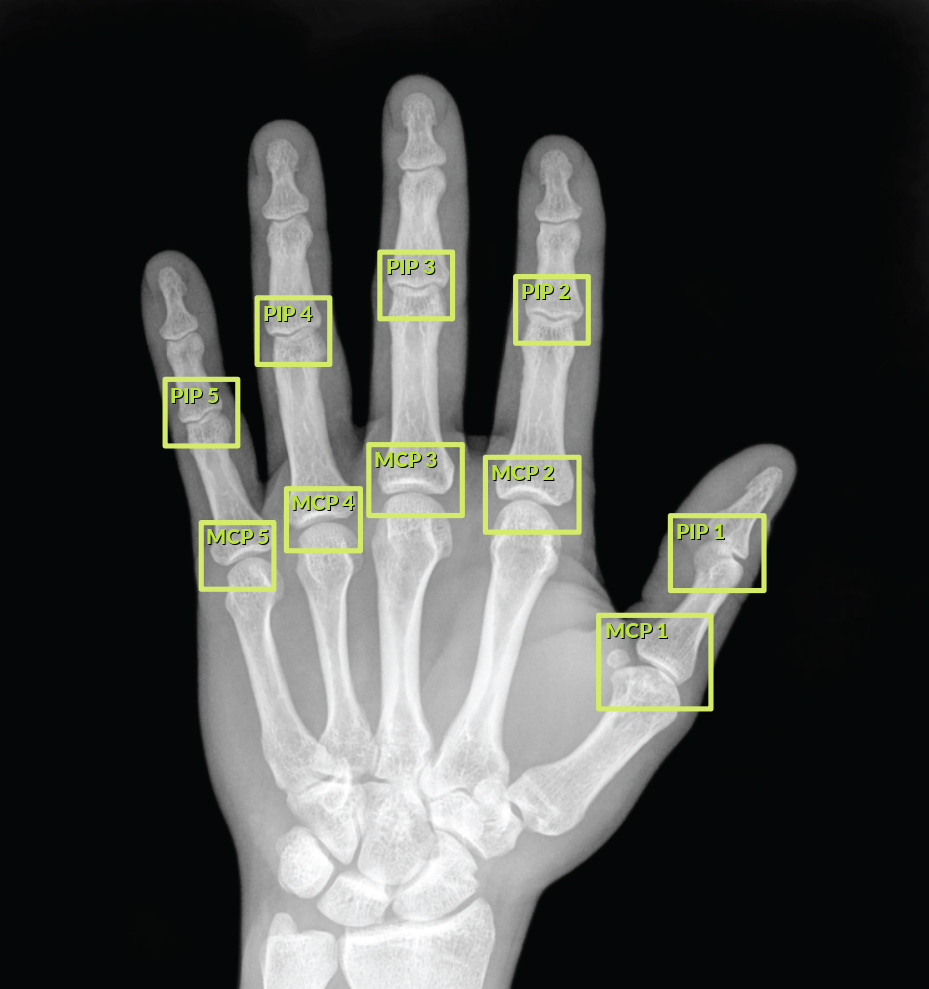
\includegraphics[width=0.4\linewidth]{pics/xray-left-hand-annotated.png}
    \caption{Röntgenbild einer linken Hand mit markierten Metacarpophalangealgelenken (MCP) und proximalen Interphalangealgelenken (PIP), Quelle: Wikimedia Commons (Lizenz: CC BY 4.0)}
    \label{fig:xray-left-hand-annotated}
\end{figure}

\section{\fontsize{14}{16}\selectfont Ergebnisse}

Das Ergebnis der Arbeit ist ein Prototyp, der einen Webservice (RESTful API) anbietet. Das Röntgenbild wird in den folgenden drei Schritten verarbeitet: Zunächst wird das auf dem Röntgenbild dargestellte Körperteil erkannt. Handelt es sich dabei um eine linke Hand, kann der Vorgang fortgesetzt werden. Im zweiten Schritt werden vom Röntgenbild die Metacarpophalangealgelenke (MCP) und proximalen Interphalangealgelenke extrahiert. Die Bildausschnitte werden an den nächsten Verarbeitungsschritt weitergereicht. Im dritten Schritt wird die Erosion der Gelenke auf einer Skala von 0 (keine Schädigung) bis 5 (Schädigung von 80 bis 100 Prozent des Gelenkgewebes) ermittelt. Die Scoring-Ergebnisse werden gesammelt und an den Client zurückgeliefert.

Dem Webservice kann via HTTP ein Röntgenbild einer linken Hand übergeben werden, worauf er in Sekundenschnelle mit einem Scoring der Metacarpophalangealgelenke (MCP) und proximalen Interphalangealgelenke im JSON-Format antwortet:

\begin{lstlisting}
$ curl -k -X POST -F "xray=@hand-left.jpg" https://localhost:8080/score | jq
{
  "scores": {
    "mcp1": 1, "mcp2": 0, "mcp3": 1, "mcp4": 1, "mcp5": 1,
    "pip1": 1, "pip2": 3, "pip3": 2, "pip4": 5, "pip5": 5
  }
}
\end{lstlisting}

\section{\fontsize{14}{16}\selectfont Lösungskonzept}

Die genannten Schritte sollen in einer für den Client nützlichen Frist ausgeführt werden. Wird erst mit dem Scoring begonnen, wenn \textit{alle} Gelenke extrahiert worden sind, dauert dies recht lange. Darum arbeitet der Prototyp asynchron, sodass mit dem Scoring bereits begonnen werden kann, wenn das \textit{erste} Gelenk extrahiert worden ist. Hierzu werden die verschiedenen Komponenten (siehe \imgref{fig:architektur}) lose mittels Messaging gekoppelt, sodass diese mit mehreren Instanzen ausgeführt werden können. Dadurch kann die Extraktion und das Scoring mehrerer Gelenke parallel ausgeführt werden, was sich positiv auf die Performance auswirkt.

Eine Orchestrator-Komponente koordiniert den ganzen Ablauf und die Kommunikation mit dem Client. Kann auf einem gegebenen Röntgenbild eine linke Hand erkannt werden, gibt der Orchestrator die Extraktion der Gelenke in Auftrag. Diese Anfragen werden mit einem \textit{Correlation Identifier} ausgestattet. Die extrahierten Gelenke werden via Queue, d.h. am Orchestrator vorbei an das Scoring geschickt. Der Orchestrator sammelt die Scores über eine weitere Queue ein, und kann diese anhand ihres Correlation Identifiers dem richtigen Client zuordnen.

\begin{figure}
    \centering
    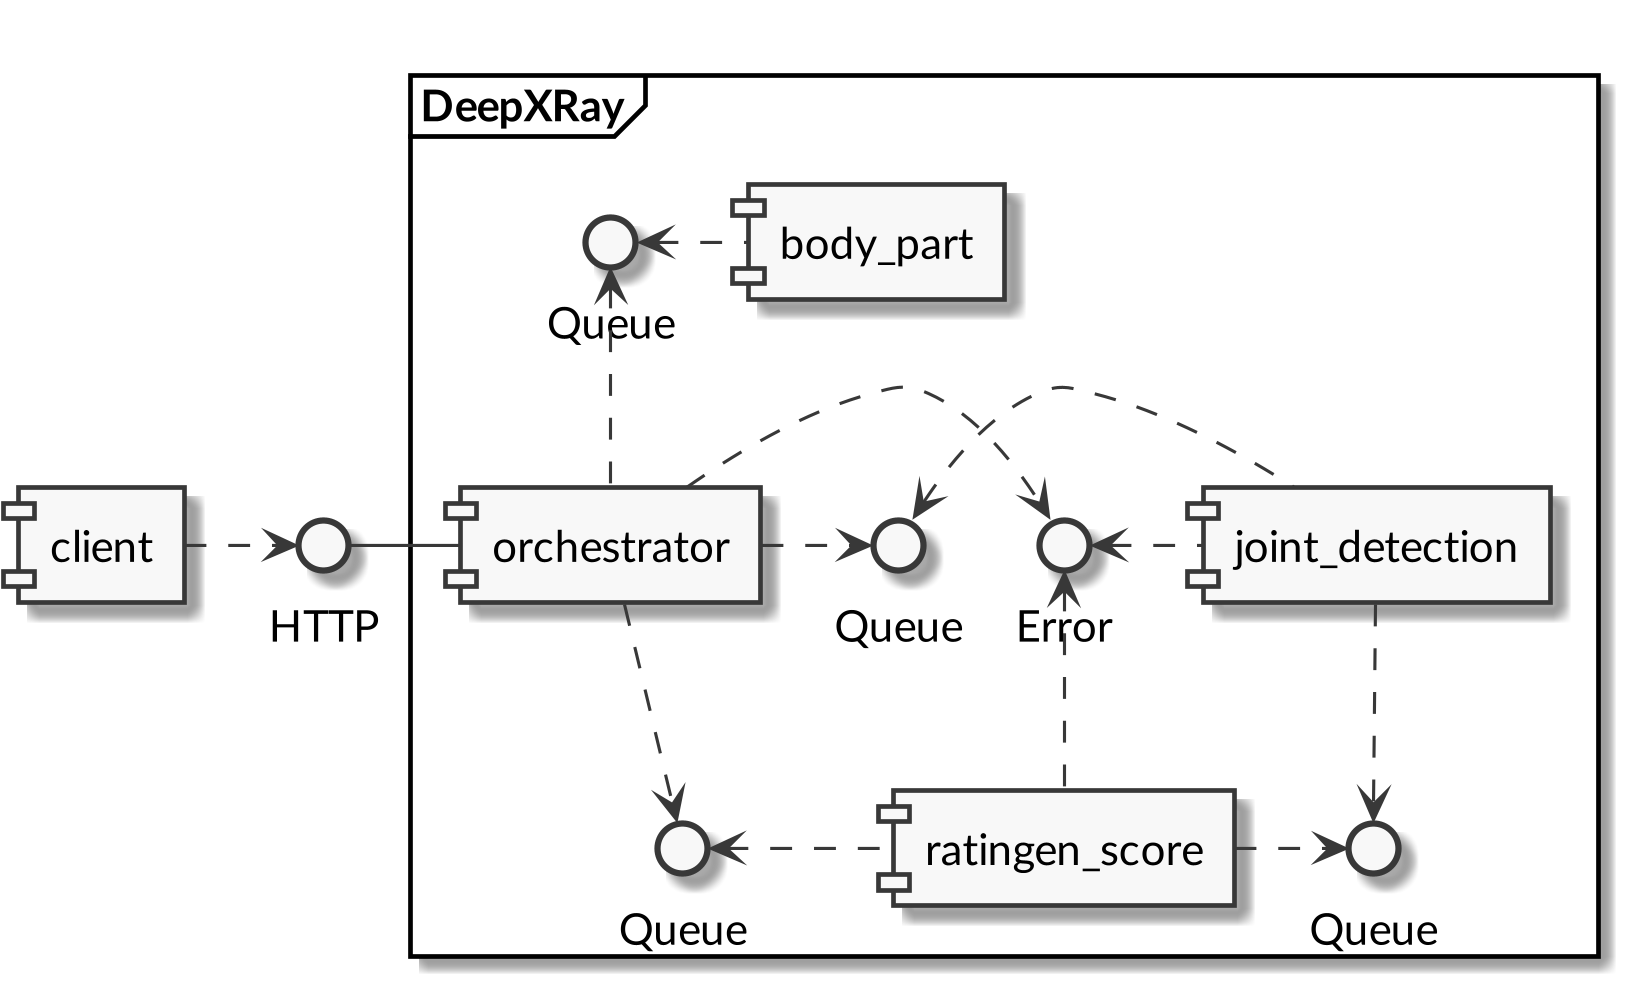
\includegraphics[width=0.6\linewidth]{../doc/pics/architektur-variante-queue-2.png}
    \caption{Die Architektur des Prototyps, die eine performante Verarbeitung von Röntgenbildern ermöglicht. Die einzelnen Komponenten sind lose via Messaging gekoppelt.}
    \label{fig:architektur}
\end{figure}

\section{\fontsize{14}{16}\selectfont Spezielle Herausforderungen}

Die Machine-Learning-Modelle waren mit verschiedenen Frameworks in unterschiedlichen Versionen entwickelt worden (TensorFlow 0.12, TensorFlow 1.4, Keras usw.). Eine Konvertierung der Modelle für neuere Versionen war für den gegebenen Projektrahmen zu aufwändig. Dadurch ist die Ausführung der Modelle nicht in einer einheitlichen Laufzeitumgebung möglich. Die Modelle werden darum isoliert in Containern ausgeführt.

Der Prototyp muss gegen aussen eine synchrone API anbieten, welche die Röntgenbilder in einer nützlichen Frist, d.h. in Sekundenschnelle verarbeiten kann. Hierzu muss das System intern asynchron arbeiten, um eine nebenläufige Abarbeitung der einzelnen Schritte zu ermöglichen, und um so die nötige Performance gewährleisten zu können.

Weiter mussten für das Spezialgebiet der Rheumaforschung sinnvolle Evaluationsmetriken gefunden und umgesetzt werden, womit die Qualität des Gesamtsystems sinnvoll bewertet werden kann. Hierzu mussten Testdaten gesammelt, aufbereitet und manuell aussortiert werden.

\section{\fontsize{14}{16}\selectfont Ausblick}

Um den Prototyp in den Produktivbetrieb überführen zu können, sind noch einige Aufgaben zu erledigen. Die verschiedenen Modellkomponenten müssen auf performanten Servern (idealerweise mit vielen CPUs) bereitgestellt werden. Die RESTful API des Orchestrators benötigt Schutz vor unbefugtem Zugriff, wozu geeignete Mechanismen (wie z.B. OAuth 2.0) einzurichten sind. Die Kommunikation zwischen dem Client und dem Orchestrator muss mit einem «richtigen», d.h. nicht selbst signierten TLS-Zertifikat abgesichert werden. Schliesslich muss der Service in andere Anwendungen integriert werden.

Die Machine-Learning-Modelle sollten längerfristig auf die aktuelle Version von TensorFlow migriert werden. Mit dem weit verbreiteten \textit{SavedModel}-Format kann sichergestellt werden, dass die Modelle auch in Zukunft unterstützt und in verschiedenen Umgebungen ausgeführt werden können. Der Einfluss der aktualisierten Modelle auf die Qualität des Gesamtsystems kann mithilfe der bereitgestellten Evaluationsmechanismen überprüft werden. Längerfristig sollen nebst linken Händen auch andere Körperteile verarbeitet werden können, wozu die Modelle entsprechend zu erweitern sind.

\end{document}
